Le cas des quadrilatères a montré que la convexité était un ingrédient central. Ceci sera aussi le cas pour les \ngones, bien que moins immédiat à justifier, comme nous le verrons dans le fait \ref{max-is-conv}, dont la preuve est indépendante des résultats de cette section.
%
Ceci explique que nous allons chercher à justifier l'existence d'au moins un \ngone\ convexe d'aire maximale parmi les \ngones\ convexes de longueur fixée. Nous allons presque y arriver...
Pour ce faire, commençons par vérifier que notre définition d'un \ngone\ convexe correspond bien à ce que nous connaissions des polygones convexes au lycée.


% ----------------------- %


\begin{fact} \label{conv-pos-det}
    Pour tout \ngone\ convexe $\setproba{P} = A_1 A_2 \cdots A_n$, l'une des alternatives suivantes a lieu.
    %
	\begin{itemize}
		\item $\forall (i, k) \in \ZintervalC{1}{n}^2$,
		si $k \notin \setgene{i ; i+1}$, alors
		$\det \big( \vect{A^{\,\prime}_i A^{\,\prime}_{i+1}}, \vect{A^{\,\prime}_i A^{\,\prime}_k} \big) > 0$.

		\item $\forall (i, k) \in \ZintervalC{1}{n}^2$,
		si $k \notin \setgene{i ; i+1}$, alors
		$\det \big( \vect{A^{\,\prime}_i A^{\,\prime}_{i+1}}, \vect{A^{\,\prime}_i A^{\,\prime}_k} \big) < 0$.
    \end{itemize}
\end{fact}


\begin{proof}
	Le cas $n = 3$ des triangles est immédiat.
	On considère alors $\setproba{P}$ un \ngone\ convexe où  $n \geq 4$.
	Nous savons que, relativement à $\setproba{P}$, les sommets sont distincts deux à deux, et qu'aucun triplet de sommets consécutifs alignés n'existe.
	Dès lors, dans le plan orienté, les trois premiers sommets sont placés suivant l'une des deux configurations suivantes. 
    
    \begin{multicols}{2}
        \small\itshape\centering
       	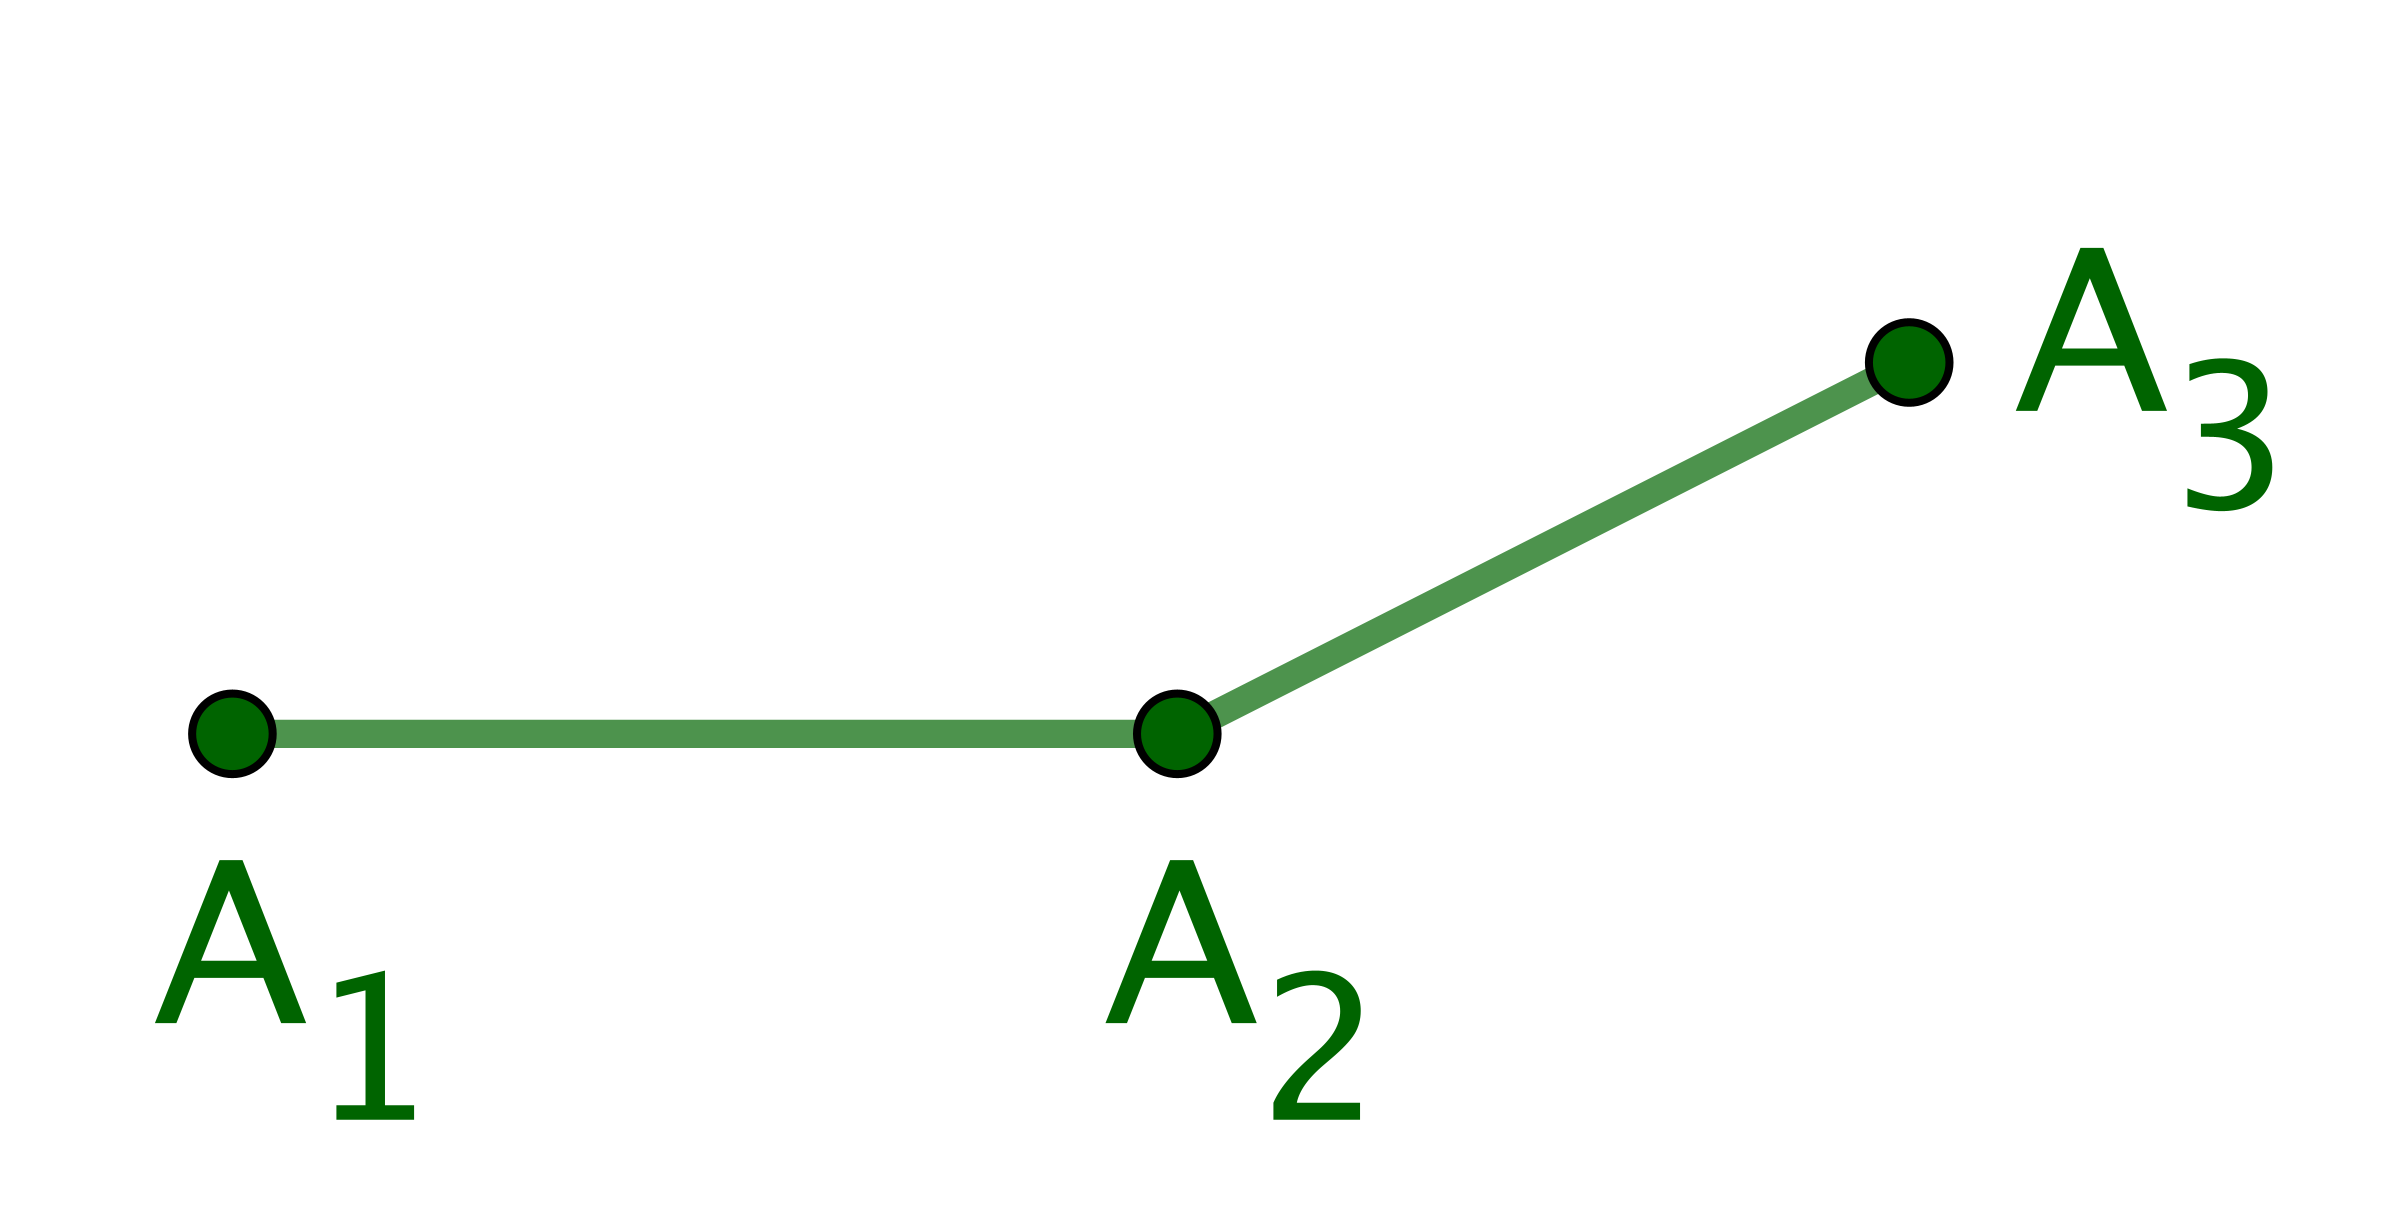
\includegraphics[scale=.45]{content/polygon/at-least-one/conv-det-sign-1.png}
    	    
    	\smallskip
        Cas positif.
        
        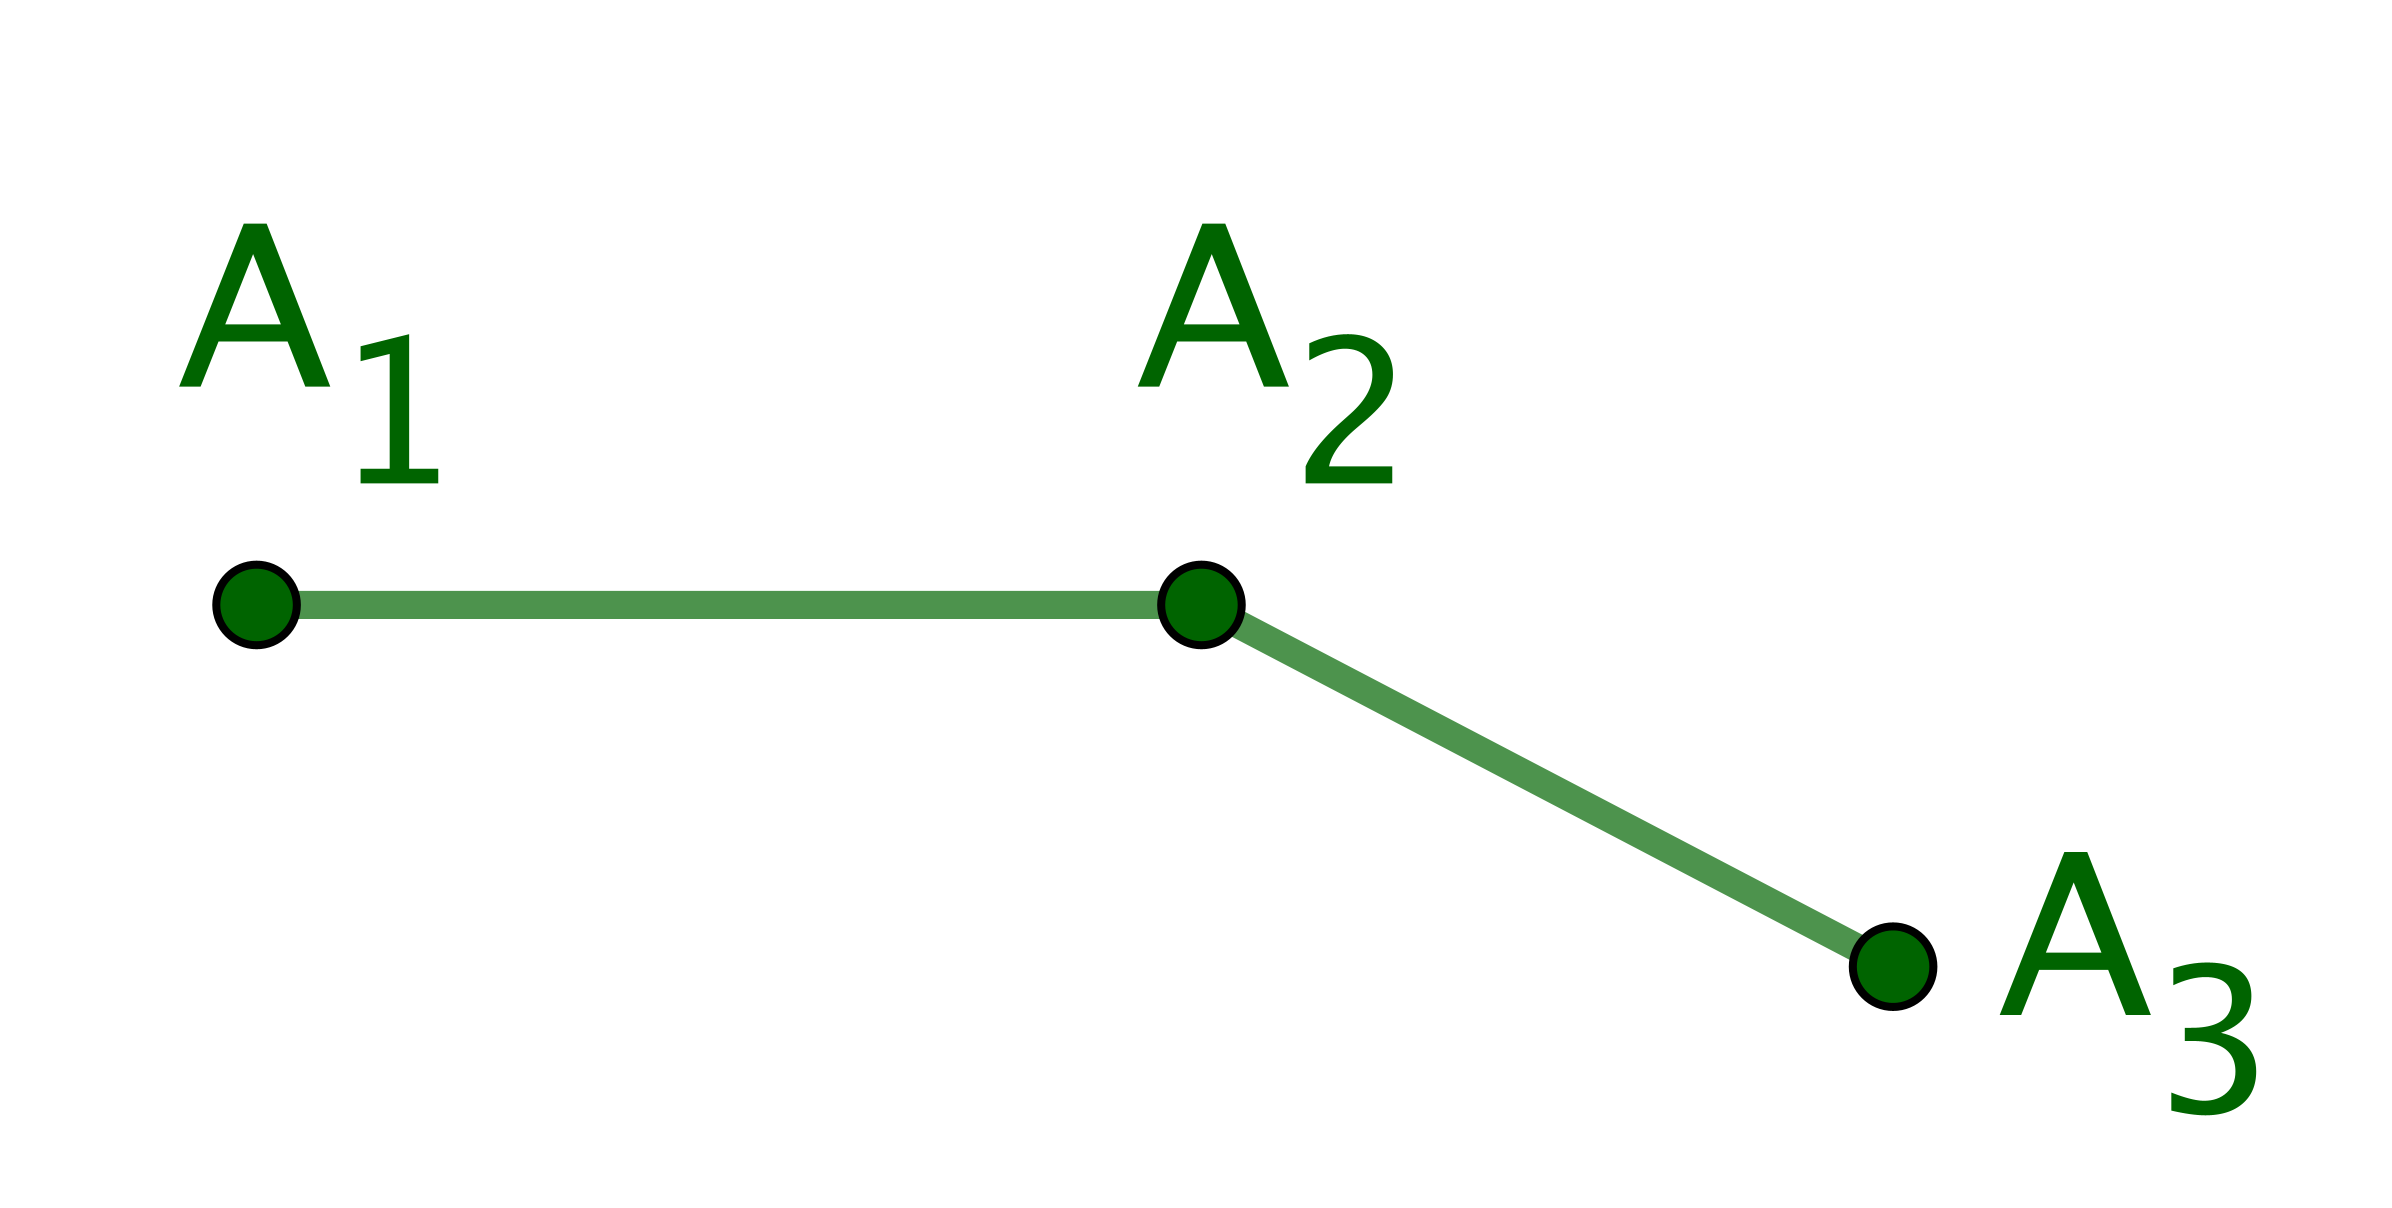
\includegraphics[scale=.45]{content/polygon/at-least-one/conv-det-sign-2.png}
    	    
    	\smallskip
        Cas négatif.
    \end{multicols}

    
    \noindent
    Considérons le cas positif, c'est-à-dire supposons que 
    $\det \big( \vect{A^{\,\prime}_1 A^{\,\prime}_2}, \vect{A^{\,\prime}_1 A^{\,\prime}_3} \big) > 0$.
	%
	\begin{itemize}
    	\item $\vect{A^{\,\prime}_1 A^{\,\prime}_3} = \vect{A^{\,\prime}_1 A^{\,\prime}_2} + \vect{A^{\,\prime}_2 A^{\,\prime}_3}$
    	donne
		$\det \big( \vect{A^{\,\prime}_2 A^{\,\prime}_3}, \vect{A^{\,\prime}_2 A^{\,\prime}_1} \big) > 0$.


		\item Comme $A_2$, $A_3$ et $A_4$ ne sont pas alignés, et de plus $A_1$ et $A_4$ du même côté, au sens large, de la droite $(A_2 A_3)$, nous obtenons
		$\det \big( \vect{A^{\,\prime}_2 A^{\,\prime}_3}, \vect{A^{\,\prime}_2 A^{\,\prime}_4} \big) > 0$.


		\item En continuant de proche en proche, nous arrivons à
		$\det \big( \vect{A^{\,\prime}_i A^{\,\prime}_{i+1}}, \vect{A^{\,\prime}_i A^{\,\prime}_{i+2}} \big) > 0$
		pour $i \in \ZintervalC{1}{n}$ quelconque.


		\item Le point précédent et la convexité donnent
		$\det \big( \vect{A^{\,\prime}_i A^{\,\prime}_{i+1}}, \vect{A^{\,\prime}_i A^{\,\prime}_k} \big) \geq 0$
		pour $(i, k) \in \ZintervalC{1}{n}^2$ tel que $k \notin \setgene{i ; i+1}$.


		\item
		Montrons maintenant que
		$\det \big( \vect{A^{\,\prime}_1 A^{\,\prime}_2}, \vect{A^{\,\prime}_1 A^{\,\prime}_k} \big) > 0$
		pour $k \in \ZintervalC{3}{n}$.
		%
		Nous savons déjà l'inégalité vraie pour $k = 3$, donc passons à $k = 4$.
		Pour avoir 
		$\det \big( \vect{A^{\,\prime}_1 A^{\,\prime}_2}, \vect{A^{\,\prime}_1 A^{\,\prime}_k} \big) > 0$, 
		le point précédent donne qu'il faut vérifier que 
		$\det \big( \vect{A^{\,\prime}_1 A^{\,\prime}_2}, \vect{A^{\,\prime}_1 A^{\,\prime}_k} \big) = 0$
		est impossible.
		Supposons donc l'égalité vraie, ce qui implique d'avoir $n \geq 5$, et donne les configurations suivantes où les hachures et la droite en trait plein sont des zones interdites pour $A_4$.

        \begin{multicols}{2}
            \small\itshape\centering
           	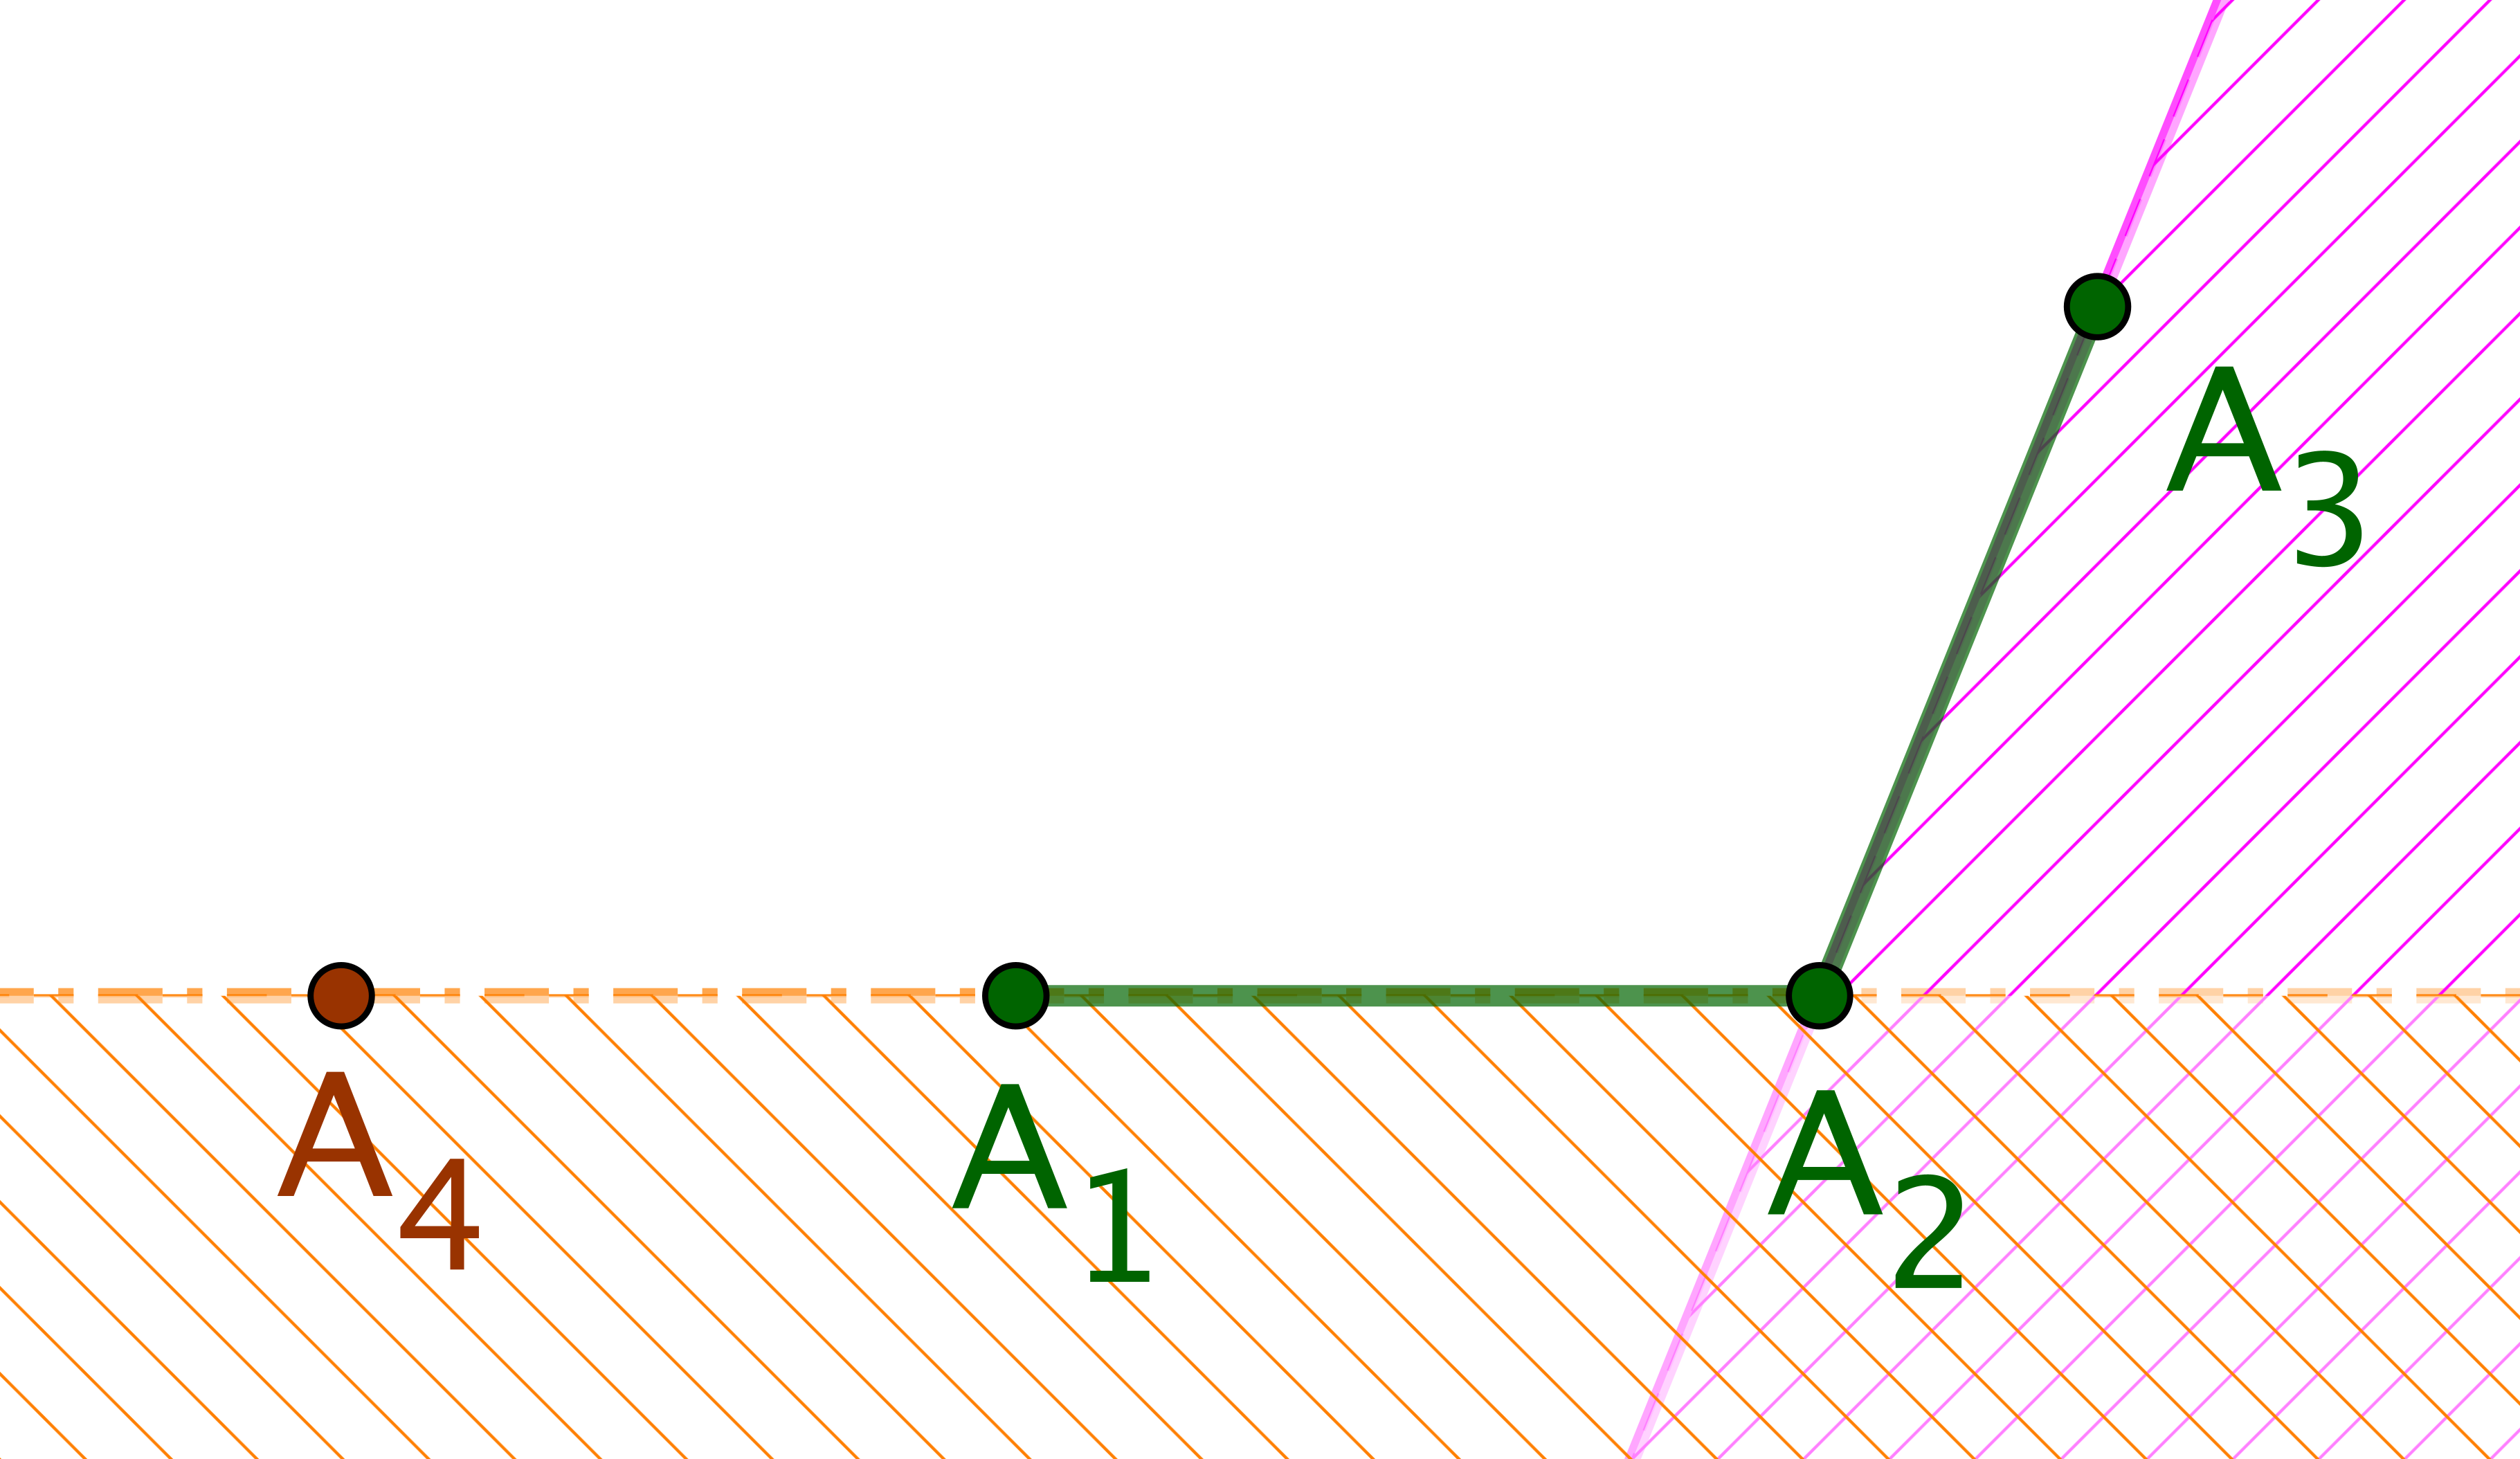
\includegraphics[scale=.4]{content/polygon/at-least-one/conv-det-A4-1.png}
        	    
        	\smallskip
            Cas 1.
            
            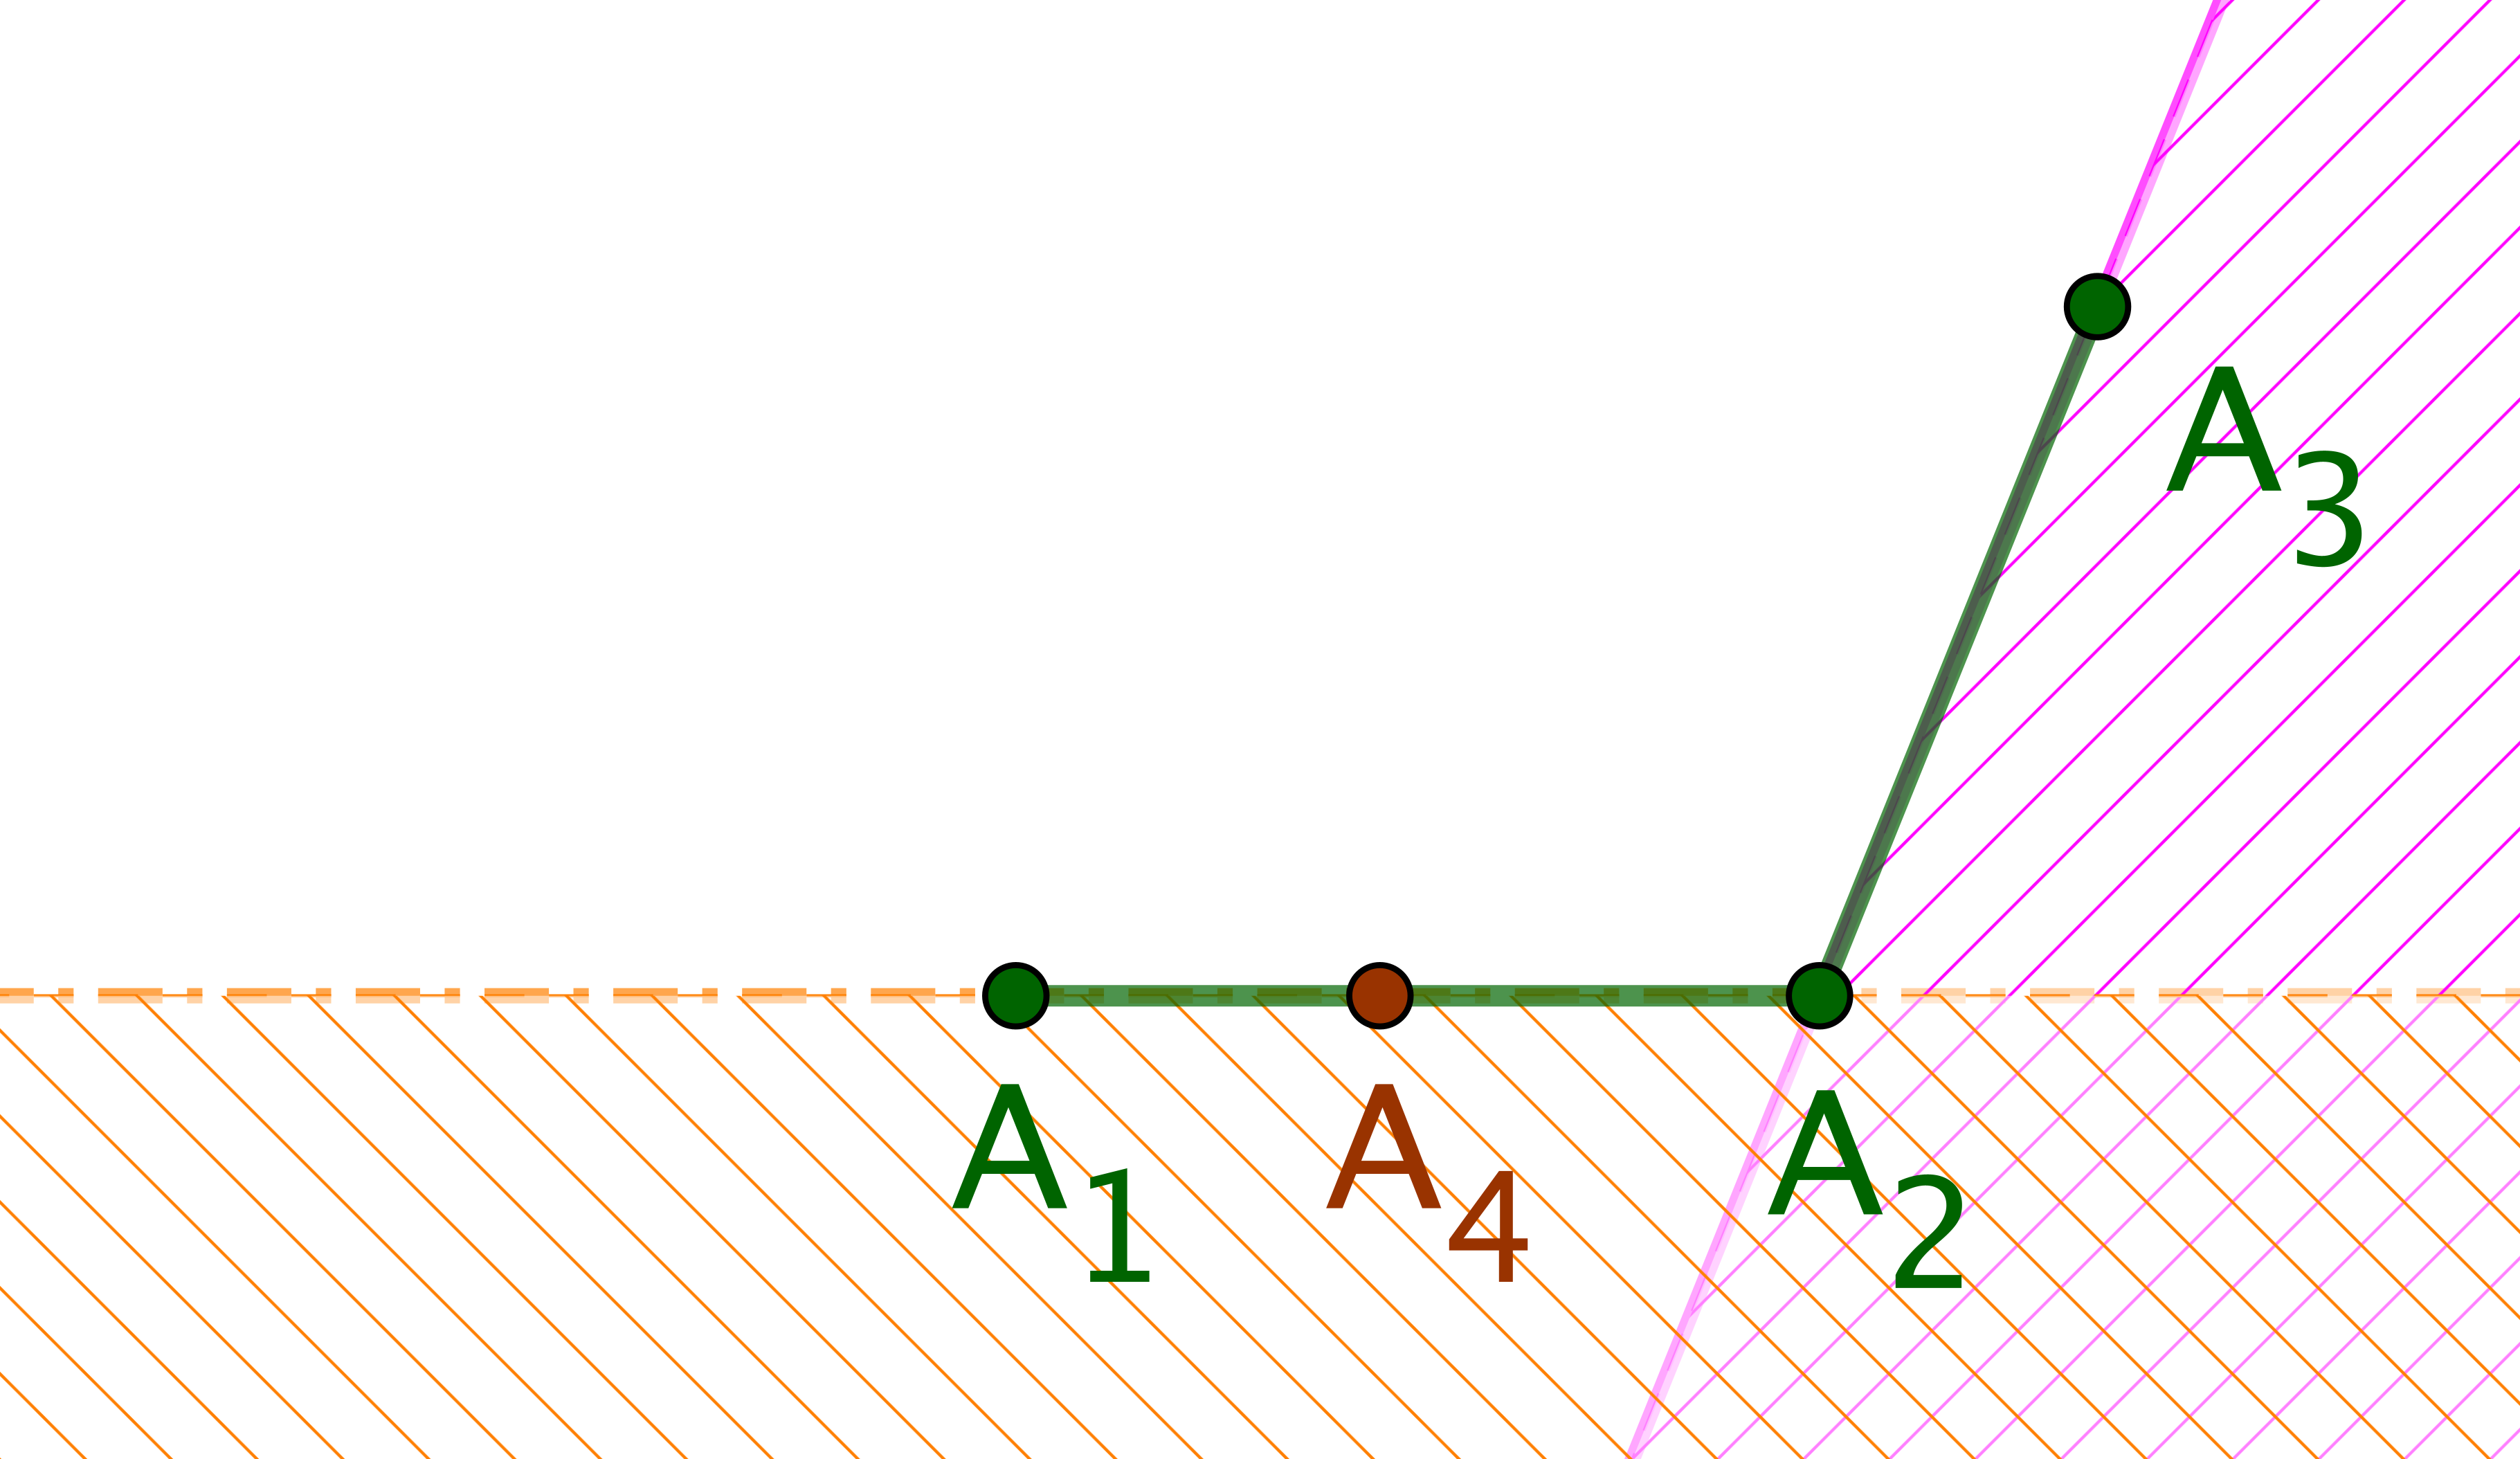
\includegraphics[scale=.4]{content/polygon/at-least-one/conv-det-A4-2.png}
        	    
        	\smallskip
            Cas 2.
        \end{multicols}
    
		\noindent
		Le cas 2 est impossible par raison de convexité, car $A_1$ et $A_2$ sont de part et d'autre de la droite $(A_3 A_4)$. Voyons donc ce qu'implique le 1\ier\ cas pour $A_5$.
		
        \begin{multicols}{2}
            \small\itshape\centering
           	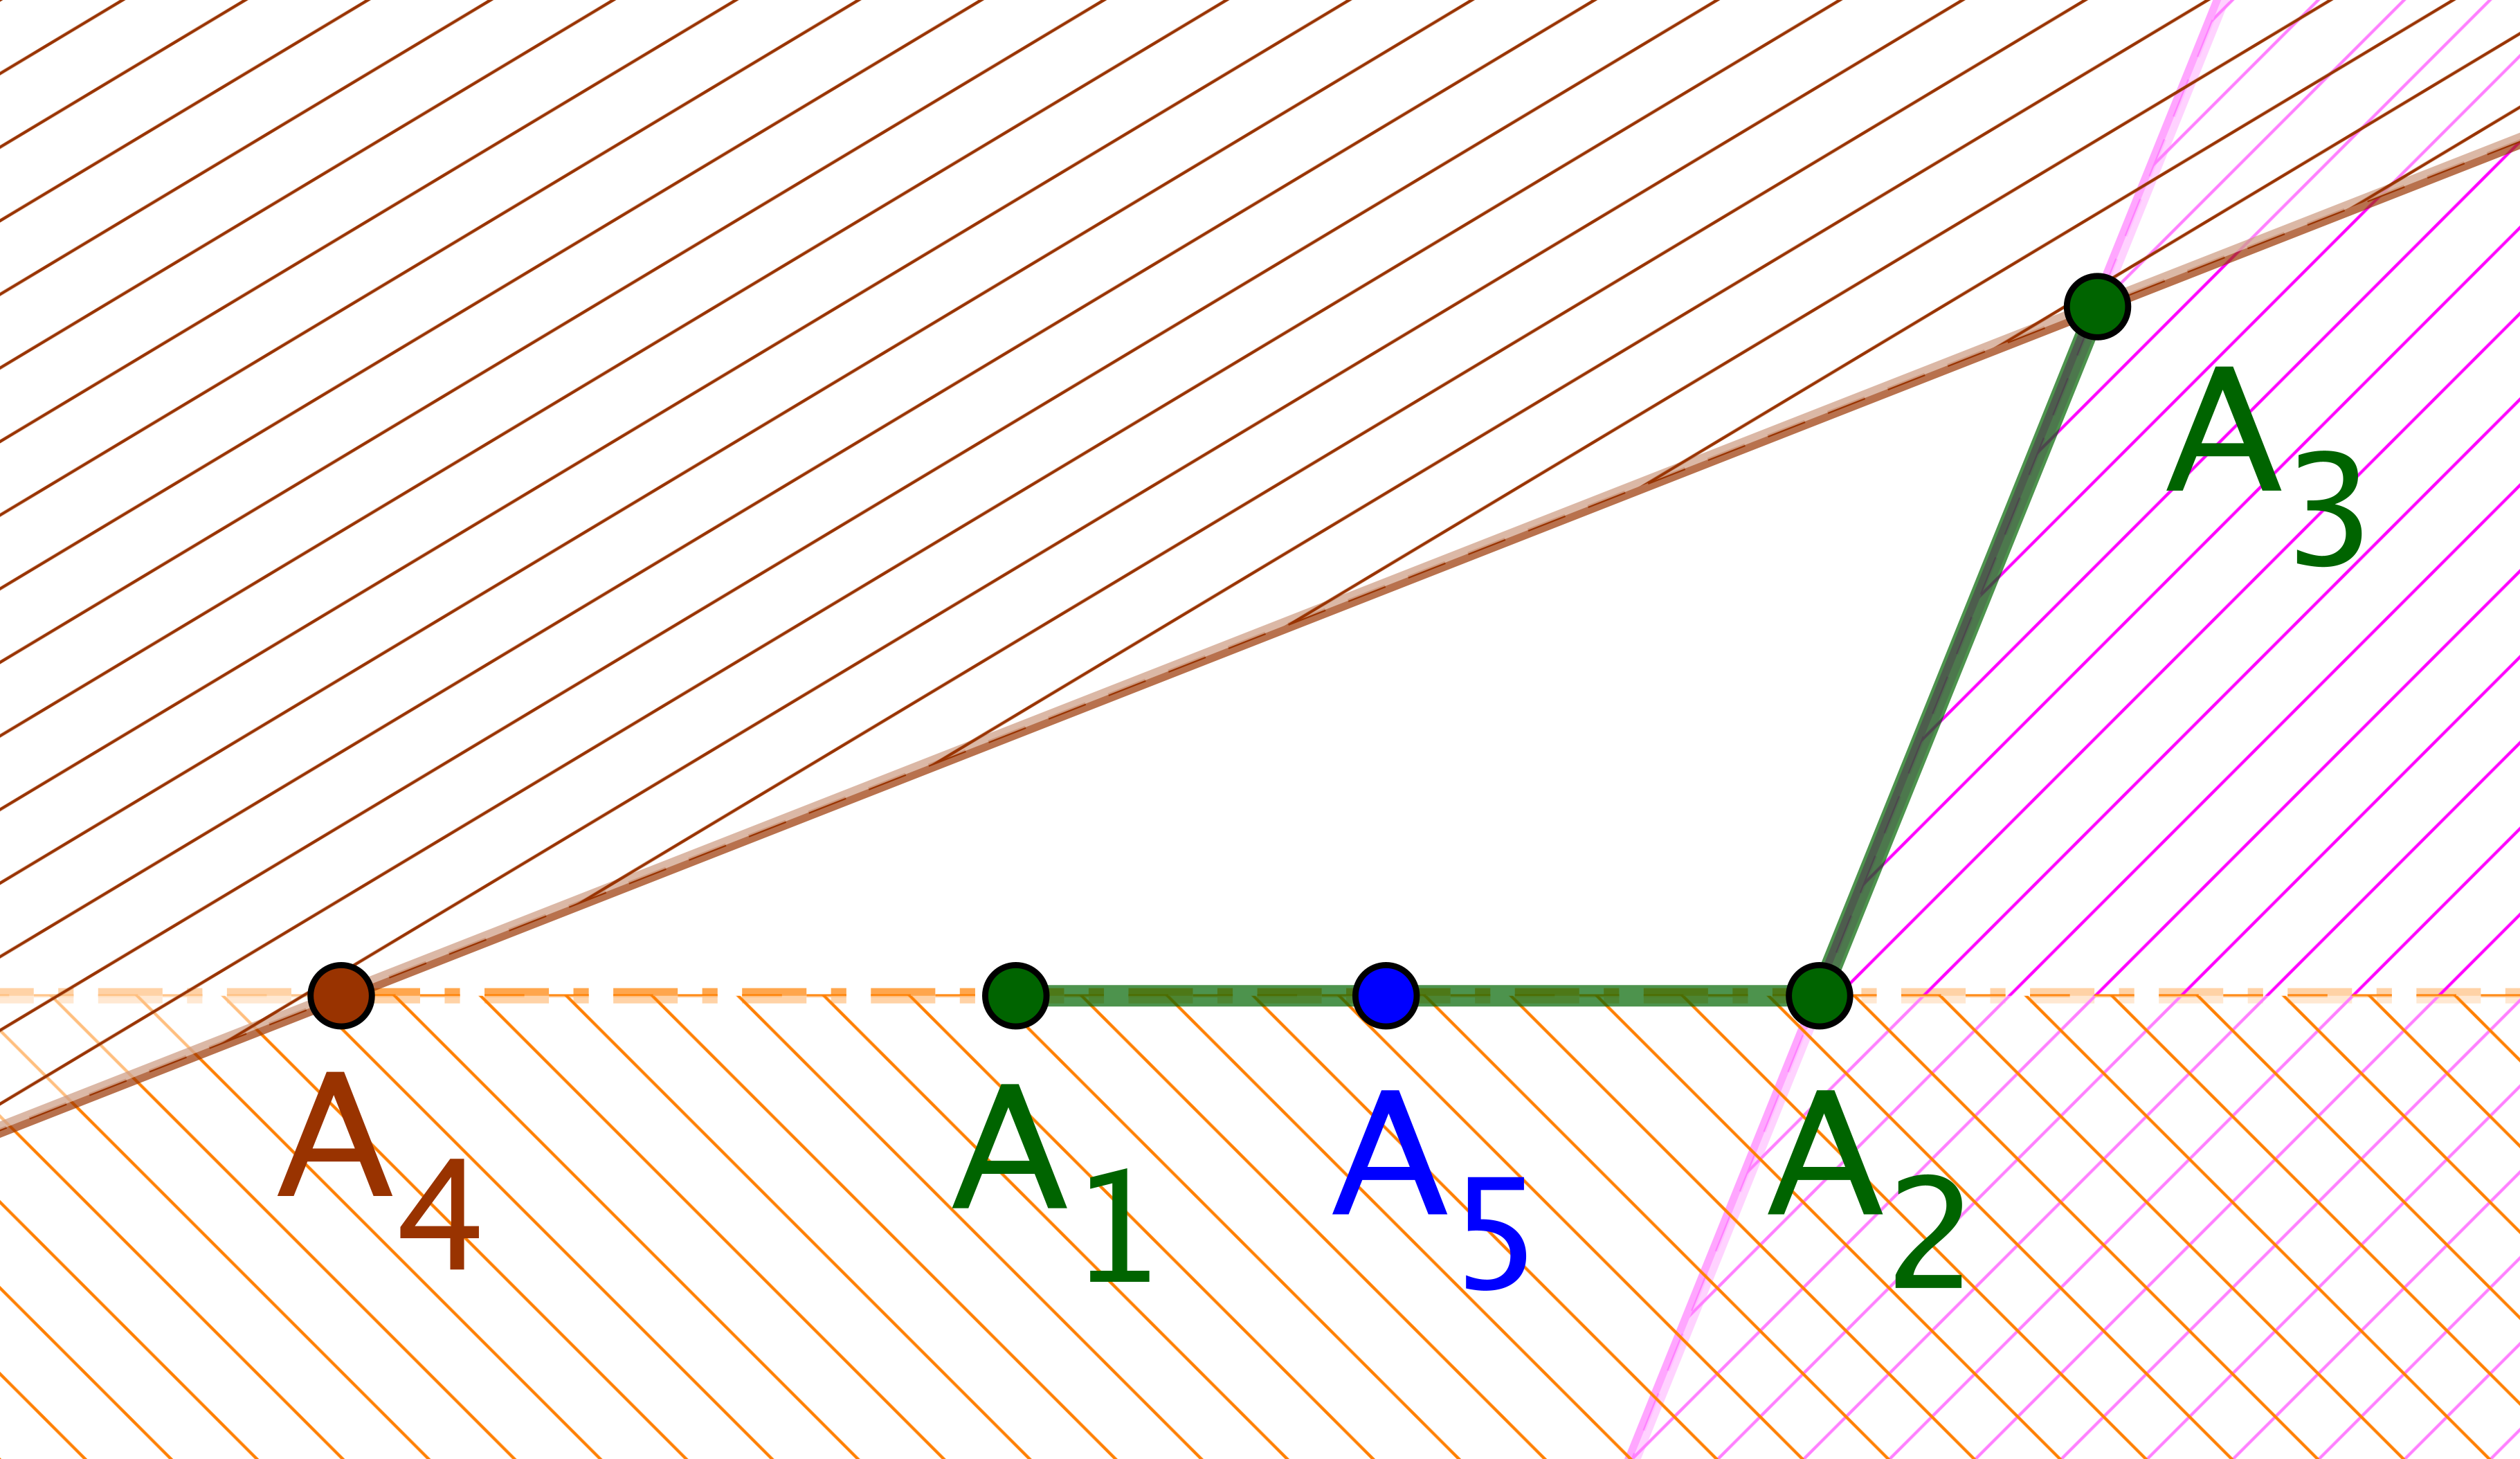
\includegraphics[scale=.4]{content/polygon/at-least-one/conv-det-A5-1.png}
        	    
        	\smallskip
            Cas 1-1.
            
            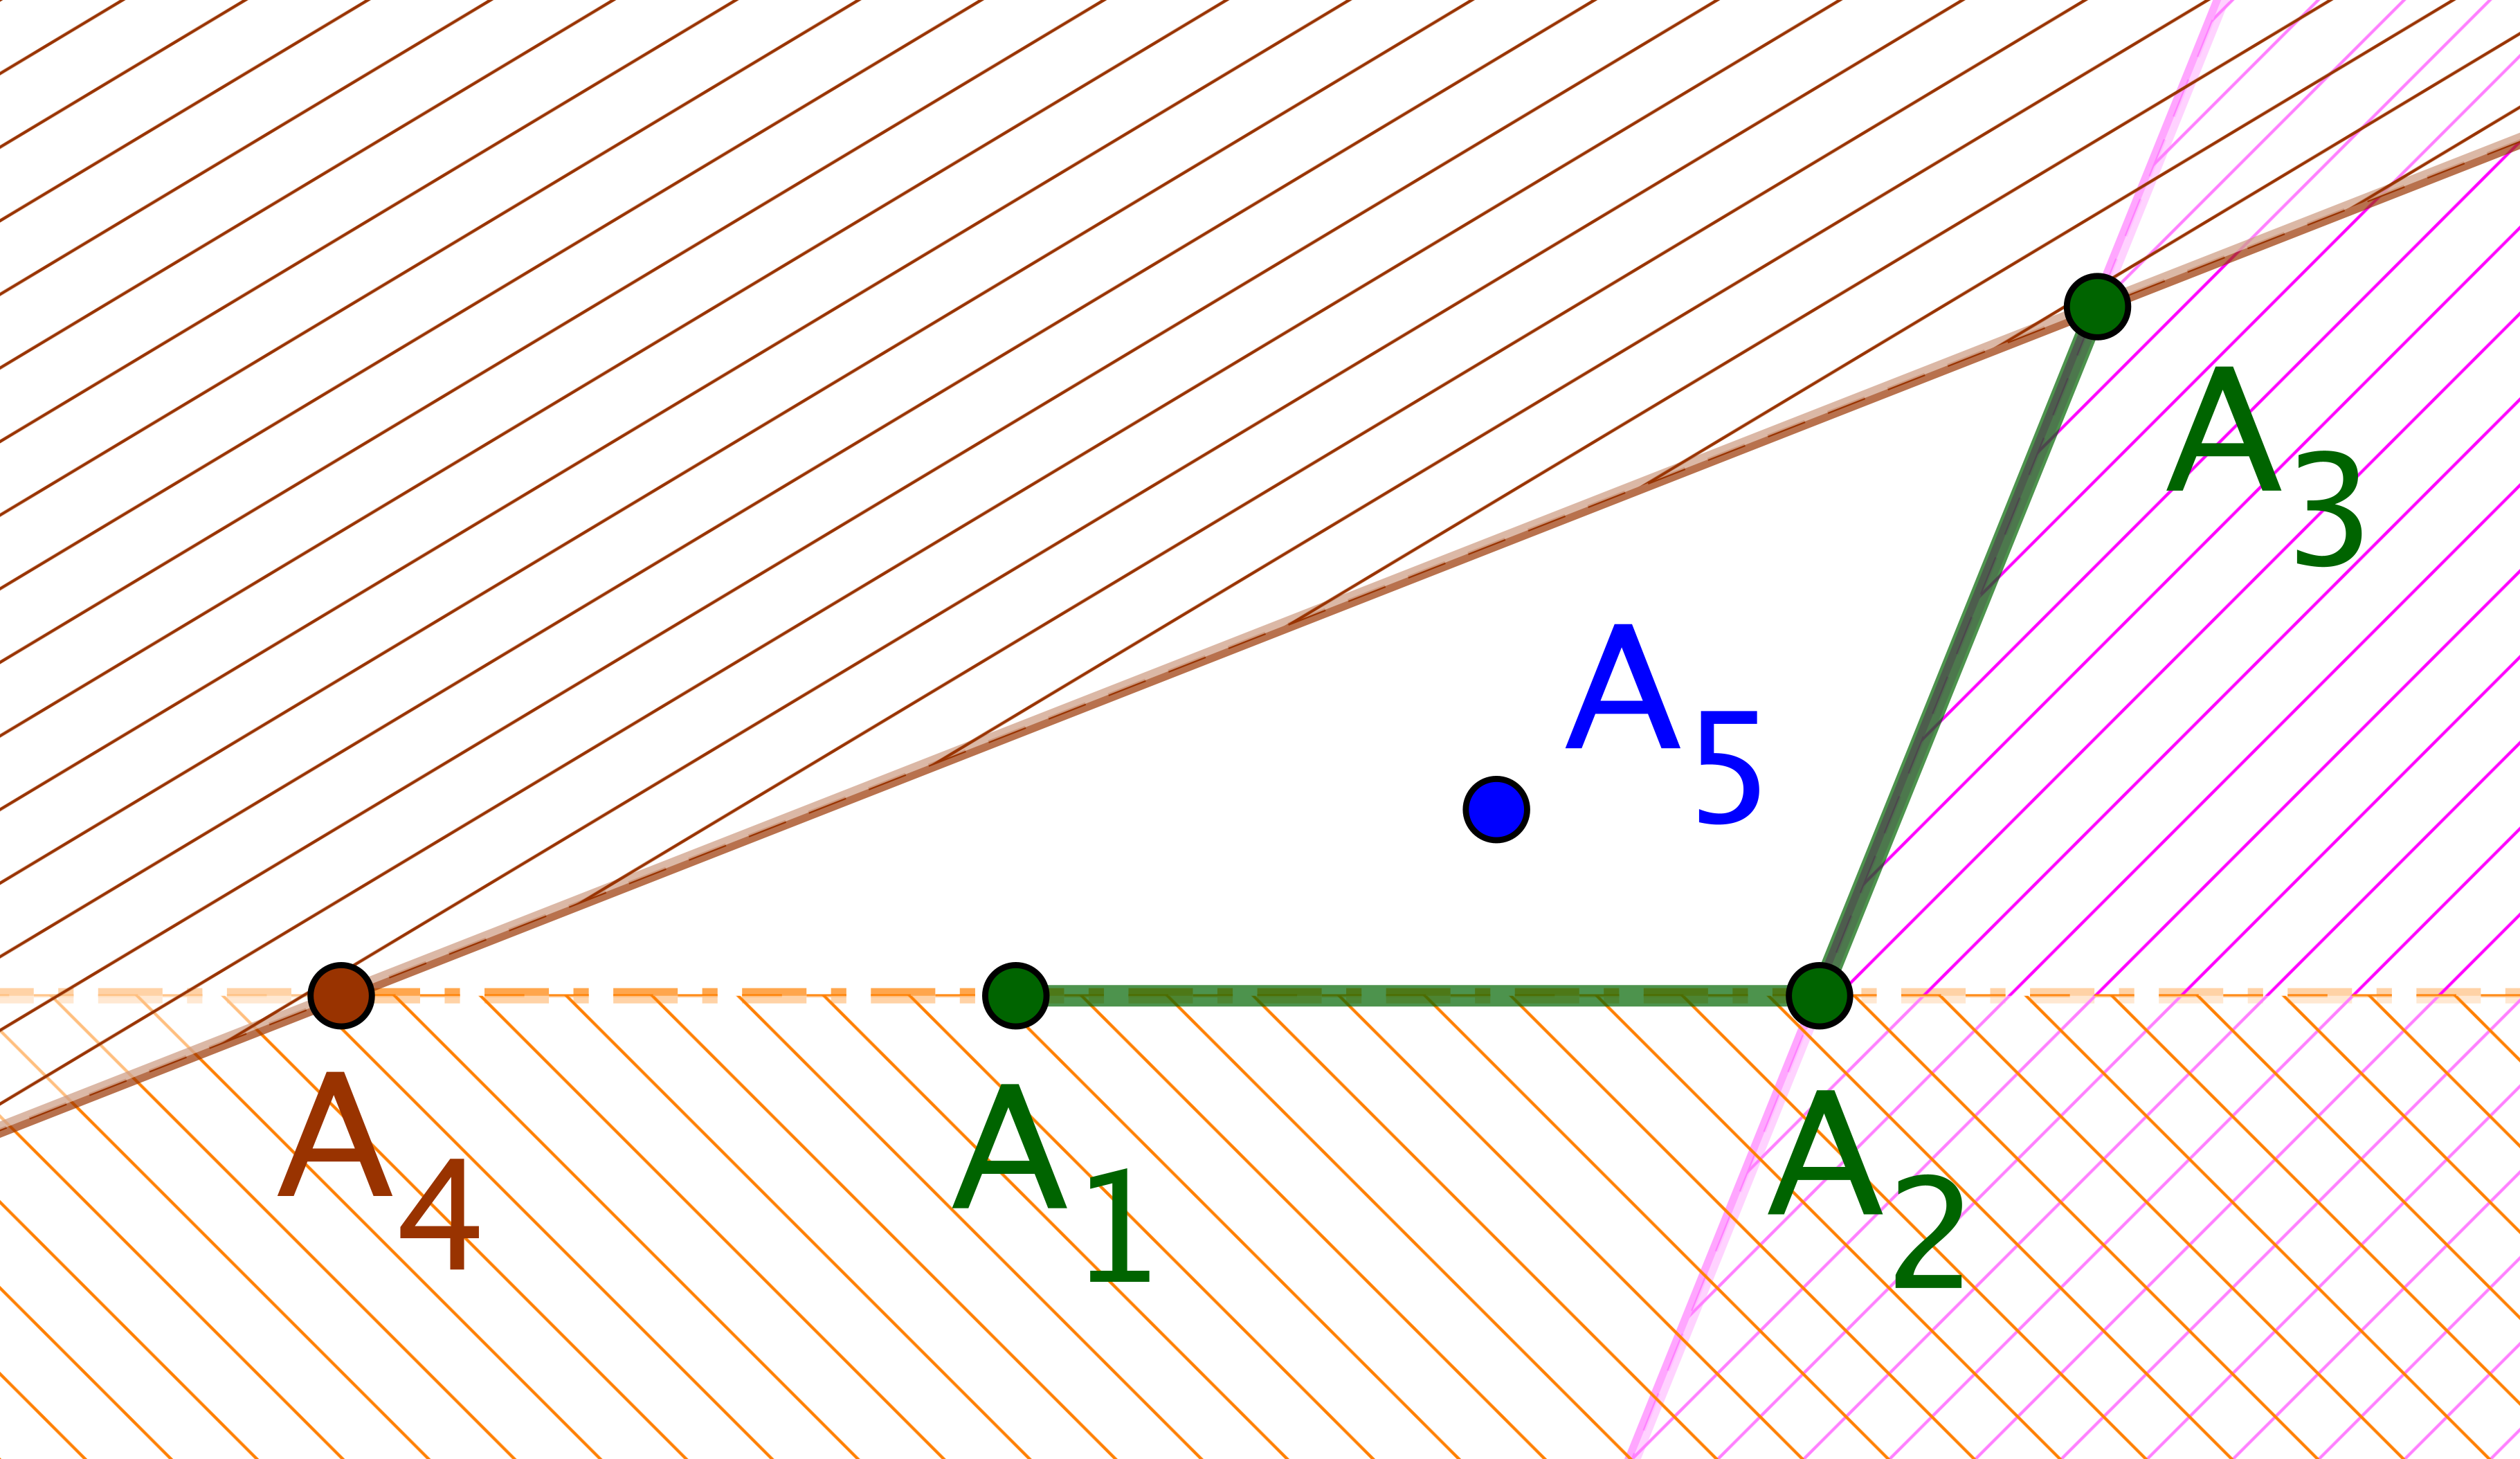
\includegraphics[scale=.4]{content/polygon/at-least-one/conv-det-A5-2.png}
        	    
        	\smallskip
            Cas 1-2.
        \end{multicols}
    
		\noindent
		Le cas 1-2 est impossible par raison de convexité à cause de $(A_4 A_5)$.
		Notons que dans le cas 1-1, il est possible d'avoir $A_5 \in ]A_4 A_1[$.
		Comme $A_5 \in (A_1 A_2)$, nous devons avoir $n \geq 6$.
		Dès lors, nous avons de nouveau $A_6 \in (A_1 A_2)$, mais ceci donne la contradiction $A_6 \in (A_4 A_5)$.
		Continuons ensuite de proche en proche, nous obtenons bien
		$\det \big( \vect{A^{\,\prime}_1 A^{\,\prime}_2}, \vect{A^{\,\prime}_1 A^{\,\prime}_k} \big) > 0$
		pour $k \in \ZintervalC{3}{n}$.


		\item En généralisant le raisonnement précédent,%
		\footnote{
		    Se souvenir de la définition de la suite $(A^{\,\prime}_i)$.
		}
		nous avons
		$\det \big( \vect{A^{\,\prime}_i A^{\,\prime}_{i+1}}, \vect{A^{\,\prime}_i A^{\,\prime}_k} \big) > 0$
		pour tout couple $(i, k) \in \ZintervalC{1}{n}^2$ vérifiant $k \notin \setgene{i ; i+1}$.
	\end{itemize}


    \noindent
    Le cas négatif se traite de façon similaire.
\end{proof}


% ----------------------- %


\newpage %TEMPO

Nous allons établir une réciproque élargie du résultat précédent. Ce nouveau fait va nous rendre un grand service par la suite.%
\footnote{
    Pourquoi s'attarder sur des inégalités larges? Parce que nous allons travailler dans un ensemble compact, et donc fermé, de \ncycles, même si cela aura pour inconvénient de ne pas garantir le caractère $n$-gonal, selon le fait \ref{conv-from-non-neg-det}, mais nous n'avons pas le choix!
}


\begin{fact} \label{conv-from-non-neg-det}
    Soit $\setproba{L} = A_1 A_2 \cdots A_n$ un \ncycle\ convexe vérifiant l'une des alternatives suivantes.
    %
	\begin{itemize}
		\item $\forall (i, k) \in \ZintervalC{1}{n}^2$,
		$\det \big( \vect{A^{\,\prime}_i A^{\,\prime}_{i+1}}, \vect{A^{\,\prime}_i A^{\,\prime}_k} \big) \geq 0$.

		\item $\forall (i, k) \in \ZintervalC{1}{n}^2$,
		$\det \big( \vect{A^{\,\prime}_i A^{\,\prime}_{i+1}}, \vect{A^{\,\prime}_i A^{\,\prime}_k} \big) \leq 0$.
    \end{itemize}
    
    Ceci implique la validité de l'une des deux assertions ci-dessous.
    %
	\begin{enumerate}[label=\roman*.]
		\item Tous les sommets de $\setproba{L}$ sont alignés, autrement dit, $\setproba{L}$ est totalement dégénéré.

		\item XXXX
    \end{enumerate}
\end{fact}


\begin{proof}
    Par symétrie des alternatives à vérifier, nous pouvons nous concentrer sur le cas positif, c'est-à-dire supposer que
    $\forall (i, k) \in \ZintervalC{1}{n}^2$,
	$\det \big( \vect{A^{\,\prime}_i A^{\,\prime}_{i+1}}, \vect{A^{\,\prime}_i A^{\,\prime}_k} \big) \geq 0$.
	%
    Supposons alors $\setproba{L}$ non totalement dégénéré, de sorte qu'il existe 
    $(i, k) \in \ZintervalC{1}{n}^2$ tel que
	$k \notin \setgene{i ; i+1}$
	et
	$\det \big( \vect{A^{\,\prime}_i A^{\,\prime}_{i+1}}, \vect{A^{\,\prime}_i A^{\,\prime}_k} \big) > 0$.
	Pour raisonner algorithmiquement, nous aurons besoin d'un ensemble $\setgeo{T}$ de sommets testés, et d'une liste $\setalge{U}$ de sommets utiles, tous les deux initialement vides.
	%
	\begin{enumerate}
    	\item XXXX


    	\item XXXX


    	\item XXXX


    	\item Prenons alors $k$ minimal.
    \end{enumerate}
    
    
    YYYY
    
    
    Quitte à changer l'origine de $\setproba{L}$, sans changer le sens de parcours des sommets, nous pouvons supposer avoir $i = 1$, et donc
		$k \in \ZintervalC{3}{n}$
		tel que
		$\det \big( \vect{A^{\,\prime}_1 A^{\,\prime}_2}, \vect{A^{\,\prime}_1 A^{\,\prime}_k} \big) > 0$.
		Lors de ce renommage, on met aussi à jour tous les noms des points contenus dans $\setgeo{T}$ et $\setalge{U}$.
\end{proof}






% ----------------------- %


\newpage %TEMPO
XXX


Le résultat qui suit est juste là pour simplifier la justification du fait \ref{at-least-one-kgone} à venir.


\begin{fact} \label{at-least-one-ncycle}
    Soient $n \in \NN_{\geq3}$,
    $\ell \in \RRsp$,
    $\pvaxes{O | i | j}$ un repère orthonormé direct du plan
    et
    $\setproba{U} \subset \RR^{2n}$ l'ensemble des uplets de coordonnées $\big( x(A_1) ; y(A_1) ; \dots ; x(A_n) ; y(A_n) \big)$ où $\setproba{L} = A_1 A_2 \cdots A_n$ désigne un \ncycle\ vérifiant les conditions suivantes.
    %
    \begin{itemize}
        \item $\cyclelen{\setproba{L}} = \ell$.
    
        \item  $\forall (i, k) \in \ZintervalC{1}{n}^2$,
		$\det \big( \vect{A^{\,\prime}_i A^{\,\prime}_{i+1}}, \vect{A^{\,\prime}_i A^{\,\prime}_k} \big) \geq 0$.
    \end{itemize}
    
    On considère alors la fonction $\alpha: \setproba{U} \rightarrow \RRp$ qui à un uplet de $\setproba{U}$ associe l'aire algébrique du \ncycle\ qu'il représente.
   	%
	Avec ces notations, la fonction $\alpha: \setproba{U} \rightarrow \RRp$ admet au moins un maximum.
\end{fact}


\begin{proof}
     $\setproba{U}$ est fermé dans $\RR^{2n}$, car les conditions le définissant le sont, et il est borné, car inclus dans la boule fermée de centre $\pt{O}$ et de rayon $\ell$,
     donc $\setproba{U}$ est un compact de $\RR^{2n}$.
     De plus, $\alpha$ est continue d'après le fait \ref{sarea-cont}.
     Finalement, par continuité et compacité, $\alpha$ admet un maximum sur $\setproba{U}$.
\end{proof}


% ----------------------- %


\newpage %TEMPO
XXX

Nous arrivons, ci-dessous, au résultat central pour les \ngones\ convexes où la perte éventuelle de sommets est un faux problème, car nous aboutirons, plus tard, à la comparaison de \kregs\ convexes pour $k$ variable, une tâche aisée, puisque le périmètre et l'aire d'un \kreg\ convexe s'expriment en fonction de $k$.


\begin{fact} \label{at-least-one-kgone}
    Soient $n \in \NN_{\geq3}$ et $\ell \in \RRsp$.
    Il existe un \kgone\ convexe $\setproba{K}$ validant les assertions suivantes.
    %
	\begin{itemize}
		\item $k \leq n$ et $\cyclelen{\setproba{K}} = \ell$.

		\item Si $\setproba{P}$ est un \ngone\ convexe tel que $\cyclelen{\setproba{P}} = \ell$, alors $\area{\setproba{P}} \leq \area{\setproba{K}}$.
    \end{itemize}
\end{fact}


\begin{proof}
    Reprenons les notations du fait \ref{at-least-one-ncycle}, et considérons $\setproba{M} \in \setproba{U}$ maximisant $\alpha$.
	%
	\begin{itemize}
		\item Une simple translation permet de se ramener au cas de \ngones\ convexes d'origine $\pt{O}$.


		\item XXXX


		\item XXXX


		\item XXXX


		\item XXXX


		\item XXXX
    \end{itemize}
    
    
    
    
    
    
    
	
	XXXX
	
	
	Commençons par chercher un \ncycle\ $\setproba{M}$ tel que $\area{\setproba{P}} \leq \area{\setproba{M}}$ pour tout \ngone\ convexe $\setproba{P}$ vérifiant $\cyclelen{\setproba{P}} = \ell$.
    
    De plus, selon le fait \ref{conv-pos-det},
    
    $\sarea{\setproba{L}^{\mathrm{op}}} = - \sarea{\setproba{L}}$ pour tout \ncycle\ $\setproba{L}$ d'après le fait \ref{nline-rota-opp}, donc nous pouvons nous concentrer sur les \ncycles\ convexes vérifiant $\det \big( \vect{A^{\,\prime}_i A^{\,\prime}_{i+1}}, \vect{A^{\,\prime}_i A^{\,\prime}_k} \big) \geq 0$ pour tous les sommets $A_i$ et $A_k$ grâce au fait précédent.
	


	\begin{itemize}
		\item Munissons le plan d'un repère orthonormé direct $\pvaxes{O | i | j}$, puis notons $\setproba{U} \subset \RR^{2n}$ l'ensemble des uplets de coordonnées $\big( x(A_1) ; y(A_1) ; \dots ; x(A_n) ; y(A_n) \big)$ où $\setproba{L} = A_1 A_2 \cdots A_n$ est un \ncycle\ vérifiant les conditions suivantes.
	    %
	    \begin{enumerate}
	    	\item $A_1 = \pt{O}$.

	    	\item $\cyclelen{\setproba{L}} = \ell$.

		    \item
		    $\forall (k, i) \in \ZintervalC{1}{n}^2$,
		    $\det \big( \vect{A^{\,\prime}_i A^{\,\prime}_{i+1}}, \vect{A^{\,\prime}_i A^{\,\prime}_k} \big) \geq 0$.
	    \end{enumerate}


        \item $\setproba{U}$ est fermé dans $\RR^{2n}$, car les conditions le définissant le sont, et il est borné, car inclus dans la boule fermée de centre $\pt{O}$ et de rayon $\ell$.
        En résumé, $\setproba{U}$ est un compact de $\RR^{2n}$.


        \item Nous définissons la fonction $\alpha: \setproba{U} \rightarrow \RRp$ qui à un uplet de $\setproba{U}$ associe l'aire algébrique du \ncycle\ qu'il représente.
        Cette fonction est continue d'après le fait \ref{sarea-cont}.
        %
        Donc, $\alpha$ admet un maximum sur $\setproba{U}$ par continuité et compacité. Affaire conclue!
        
        
        \item Reprenons les notations de la preuve du fait \ref{at-least-one-ncycle}, puis notons $\setproba{K}$ un \ncycle\ convexe maximisant la fonction $\alpha$ sur $\setproba{U}$, de sorte que $\cyclelen{\setproba{K}} = \ell$ est validée.
		%
		Il est immédiat que pour tout \ngone\ convexe $\setproba{P}$ tel que $\cyclelen{\setproba{P}} = \ell$, nous avons $\sarea{\setproba{P}} \leq \sarea{\setproba{K}}$, puis le fait \ref{sarea-ngone} donne que $\area{\setproba{P}} \leq \abs{\sarea{\setproba{K}}}$, après avoir noté que nécessairement $\sarea{\setproba{K}} \geq 0$.
		%
		Pour finir, voyons pourquoi $\setproba{K}$ est un \kgone\ convexe avec $k \leq n$, ce qui impliquera ensuite $\abs{\sarea{\setproba{K}}} = \area{\setproba{K}}$.
    \end{itemize}
	
	\null\vspace{-6ex}
\end{proof}

Affaire conclue!
